\documentclass[aspectratio=169,10pt]{beamer}
\usepackage[T1]{fontenc}
\usepackage{amsmath,amssymb,amsfonts}
\usepackage{bm}
\usepackage{tikz}
\usepackage{xcolor}
\usetikzlibrary{arrows.meta,positioning,shapes,calc}

\definecolor{parchment}{HTML}{F4E8C8}
\definecolor{paper}{HTML}{FAF1D8}
\definecolor{ink}{HTML}{1A1A1A}
\definecolor{inkgray}{HTML}{5A5A5A}
\definecolor{accentred}{HTML}{8B1A1A}
\definecolor{accentgreen}{HTML}{2D5F2C}
\definecolor{accentblue}{HTML}{1F4E79}
\definecolor{redbg}{HTML}{F7E0DE}
\definecolor{grnbg}{HTML}{E0EBDC}
\definecolor{blubg}{HTML}{DDE6EF}
\definecolor{labelbg}{HTML}{EFE0B0}

\usefonttheme{serif}
\setbeamercolor{background canvas}{bg=parchment}
\setbeamercolor{normal text}{fg=ink}
\setbeamercolor{structure}{fg=ink}
\setbeamercolor{frametitle}{fg=ink,bg=parchment}
\setbeamercolor{title}{fg=ink}
\setbeamercolor{itemize item}{fg=ink}
\setbeamercolor{itemize subitem}{fg=ink}
\setbeamercolor{item}{fg=ink}
\setbeamercolor{caption name}{fg=ink}
\setbeamertemplate{navigation symbols}{}
\setbeamertemplate{itemize item}{\textbullet}

\setbeamertemplate{frametitle}{%
  \vspace{0.30em}%
  \begin{center}%
    {\bfseries\Large\insertframetitle\par}%
    \vspace{0.28em}%
    {\color{ink}\rule{0.86\paperwidth}{0.4pt}}%
  \end{center}%
  \vspace{0.10em}%
}
\setbeamertemplate{footline}{%
  \hbox to \paperwidth{\hfil\itshape\small\insertframenumber\hspace{0.7em}}%
  \vspace{0.35em}%
}

\newcommand{\vY}{\bm{Y}}
\newcommand{\vy}{\bm{y}}
\newcommand{\vA}{\bm{A}}
\newcommand{\vB}{\bm{B}}
\newcommand{\valpha}{\bm{\alpha}}
\newcommand{\vn}{\bm{n}}
\newcommand{\vs}{\bm{s}}
\newcommand{\vW}{\bm{W}}
\newcommand{\T}{^{\mathsf T}}
\newcommand{\Hh}{^{\mathsf H}}
\newcommand{\norm}[1]{\left\lVert #1\right\rVert}
\DeclareMathOperator*{\argmin}{arg\,min}

\tikzset{
  flowbox/.style={draw=ink,fill=paper,line width=0.6pt,
                  minimum width=2.5cm,minimum height=1.0cm,
                  align=center,font=\small\bfseries,inner sep=4pt},
  smallbox/.style={draw=ink,fill=paper,line width=0.4pt,
                   minimum width=0.7cm,minimum height=0.55cm,
                   inner sep=2pt,align=center,font=\footnotesize\itshape},
  method/.style={draw=accentgreen,fill=grnbg,line width=1.0pt,
                 align=center,font=\small\bfseries,inner sep=6pt},
  issue/.style={draw=accentred,fill=redbg,line width=1.0pt,
                align=center,font=\small\bfseries,inner sep=6pt},
  idea/.style={draw=accentblue,fill=blubg,line width=1.0pt,
               align=center,font=\small\bfseries,inner sep=6pt},
  flowarr/.style={-{Stealth[length=2.5mm,width=2mm]},line width=0.7pt},
  softarr/.style={-{Stealth[length=2mm,width=1.6mm]},line width=0.5pt,color=inkgray}
}

\newcommand{\bottomnote}[1]{%
  \begin{center}{\itshape\small #1}\end{center}}

\newcommand{\papercover}[4]{%
  \begin{frame}[plain]
    \vfill
    \begin{center}
      {\bfseries\Huge #1\par}
      \vspace{0.8cm}
      {\Large #2\par}
      \vspace{0.35cm}
      {\itshape\large\color{inkgray}#3\par}
      \vspace{0.55cm}
      {\small\texttt{\detokenize{#4}}\par}
    \end{center}
    \vfill
  \end{frame}}

\newcommand{\twocolmodel}[4]{%
  \begin{columns}[T,onlytextwidth]
    \begin{column}{0.48\textwidth}#1\end{column}
    \begin{column}{0.48\textwidth}#2\end{column}
  \end{columns}
  \bottomnote{#3\\#4}}


\begin{document}

\papercover
  {Adaptive Modulation and Coding}
  {Wan, Hao Zhou, Xu, Huang, Shengli Zhou, Shi, and Cui}
  {IEEE Journal of Oceanic Engineering, 2015}
  {adaptive_modulation_coding_ofdm_uwa.pdf}

\begin{frame}{1. Core Problem}
\twocolmodel{
  \begin{itemize}\setlength{\itemsep}{0.45em}
    \item UWA channels vary with location, time, and sea conditions.
    \item Fixed modulation and coding either waste rate or fail in bad fades.
    \item The receiver needs a performance metric that predicts decoding success.
  \end{itemize}
}{
  \[
    \text{mode}
    \in
    \{(M_1,R_1),\ldots,(M_5,R_5)\}
  \]
  \[
    \widehat{\text{mode}}
    =
    f(\text{channel quality})
  \]
}{
  The system adapts the transmission mode to the channel, but only from a finite practical menu.
}{
  The key metric is effective SNR after receiver processing, not just input SNR.
}
\end{frame}

\begin{frame}{2. Effective SNR}
\begin{center}
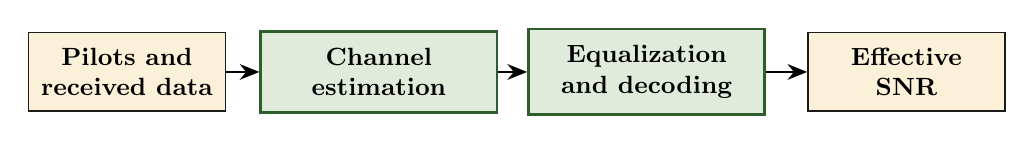
\begin{tikzpicture}[x=1cm,y=1cm]
  \node[flowbox] (pilot) at (-5.0,0) {Pilots and\\received data};
  \node[method,minimum width=3.0cm] (ce) at (-1.8,0) {Channel\\estimation};
  \node[method,minimum width=3.0cm] (dec) at (1.6,0) {Equalization\\and decoding};
  \node[flowbox] (esnr) at (4.9,0) {Effective\\SNR};
  \draw[flowarr] (pilot) -- (ce);
  \draw[flowarr] (ce) -- (dec);
  \draw[flowarr] (dec) -- (esnr);
\end{tikzpicture}
\end{center}
\[
  \mathrm{ESNR}
  \approx
  \frac{\text{post-processing signal energy}}
       {\text{noise + channel-estimation error + residual distortion}}
\]
\bottomnote{ESNR is closer to the decoder's lived reality than raw input SNR or pilot SNR.}
\end{frame}

\begin{frame}{3. AMC Loop}
\begin{enumerate}\setlength{\itemsep}{0.45em}
  \item Define a small set of tested modulation/coding modes.
  \item Estimate channel quality using recent packet reception.
  \item Compute ESNR after channel estimation and decoding.
  \item Select the highest-rate mode expected to meet the reliability target.
  \item Validate in real-time sea experiments rather than only simulation.
\end{enumerate}
\bottomnote{This paper is system-facing: it asks how receiver evidence should change the next transmission.}
\end{frame}

\begin{frame}{4. JUNA Connection}
\begin{itemize}\setlength{\itemsep}{0.5em}
  \item JUNA can expose a richer reliability metric than one-tap SNR:
  \[
    \mathrm{JUNA\ score}
    =
    g(\text{residual},\text{parity},\text{pilot fit},\text{ICI energy}).
  \]
  \item That score can drive AMC mode choice or packet-level erasure marking.
  \item Mode selection should stay finite and conservative, even if the receiver internals are sophisticated.
  \item The lesson: a receiver is also a channel-quality sensor for the transmitter.
\end{itemize}
\end{frame}

\end{document}
